\documentclass[UTF8]{ctexart}
\usepackage{algorithm}
\usepackage{algorithmic}
\usepackage{amsmath}
\usepackage{graphicx}  %插入图片
\usepackage{color} %字体颜色
\usepackage{amsfonts} % \mathbb{R}
\pdfoptionpdfminorversion=7  %插入pdf导致的版本问题
\usepackage[numbers]{natbib} %参考文献

\usepackage{geometry} % 页边距
\geometry{a4paper,left=2cm,right=2cm,top=2cm,bottom=2cm} 

%\usepackage{cite}

%\usepackage{geometry} % 页边距
%\geometry{a4paper,left=2cm,right=2cm,top=2cm,bottom=2cm} 

\renewcommand{\algorithmicrequire}{ \textbf{Input:}} %Use Input in the format of Algorithm
\renewcommand{\algorithmicensure}{ \textbf{Output:}} %UseOutput in the format of Algorithm

\title{LDP机制下的快速FIM方法}
\author{王家礼}
\date{\today}

\begin{document}
\maketitle %添加这一句才能够显示标题等信息

\begin{abstract}%摘要
this is abstract
\end{abstract}

\section{背景简介}
差分隐私,量子优越性,微型人工智能等被《麻省理工科技评论》评为2020全球十大突破技术

2020年2月26日,差分隐私技术被全球知名科技评论期刊《麻省理工学院技术评论》评为“全球十大突破性技术”,并指出该技术将被美国政府用于进行3.3 亿美国居民的2020年人口普查,同时还要对他们的身份数据进行保密。

差分隐私是密码学中的一种手段,旨在提供一种当从统计数据库查询时,最大化数据查询的准确性,同时最大限度减少识别其记录的机会。作为一种数学技术,它能够在给数据添加噪声的同时,量化计算隐私提升的程度,从而使得增加“噪音”的过程变得更加严谨。苹果和Facebook已经使用这种方法来收集聚合数据,而不需要识别特定的用户。

差分隐私技术因其独特的优势,被学术界及工业界广泛的研究,谷歌、微软、苹果等公司使用该技术在保护用户隐私的同时,手机聚合数据,从而提升服务质量。

然而,传统差分隐私技术在收集聚合数据时,用户先将原始数据提交给第三方,由第三方完成对数据的加噪处理之后,将数据发布。整个过程中,需要认定第三方是可信的。

现实生活中,找到一个可信的第三方是困难的。所以,本地化差分隐私被提出。其一方面继承了传统差分隐私技术的对敏感数据量化处理的优势,另一方面进一步细化隐私保证,将加噪过程由第三方转移至用户端,由用户独立完成对个人敏感数据的加噪处理。


\subsection{传统FP-growth算法}
传统的FP-growth算法通过两次直接扫描数据集,将用户记录信息压缩存储在频繁模式树中,用以挖掘频繁模式。如图\ref{fig:DB}为5位用户的交易记录,图\ref{fig:fptree}为所建频繁模式树。

  \begin{figure}[h]
    \centering
    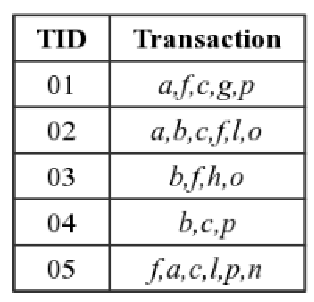
\includegraphics[width=0.3\textwidth]{DB.pdf}
    \caption{交易数据集}
    \label{fig:DB}
  \end{figure}


  \begin{figure}[h]
    \centering
    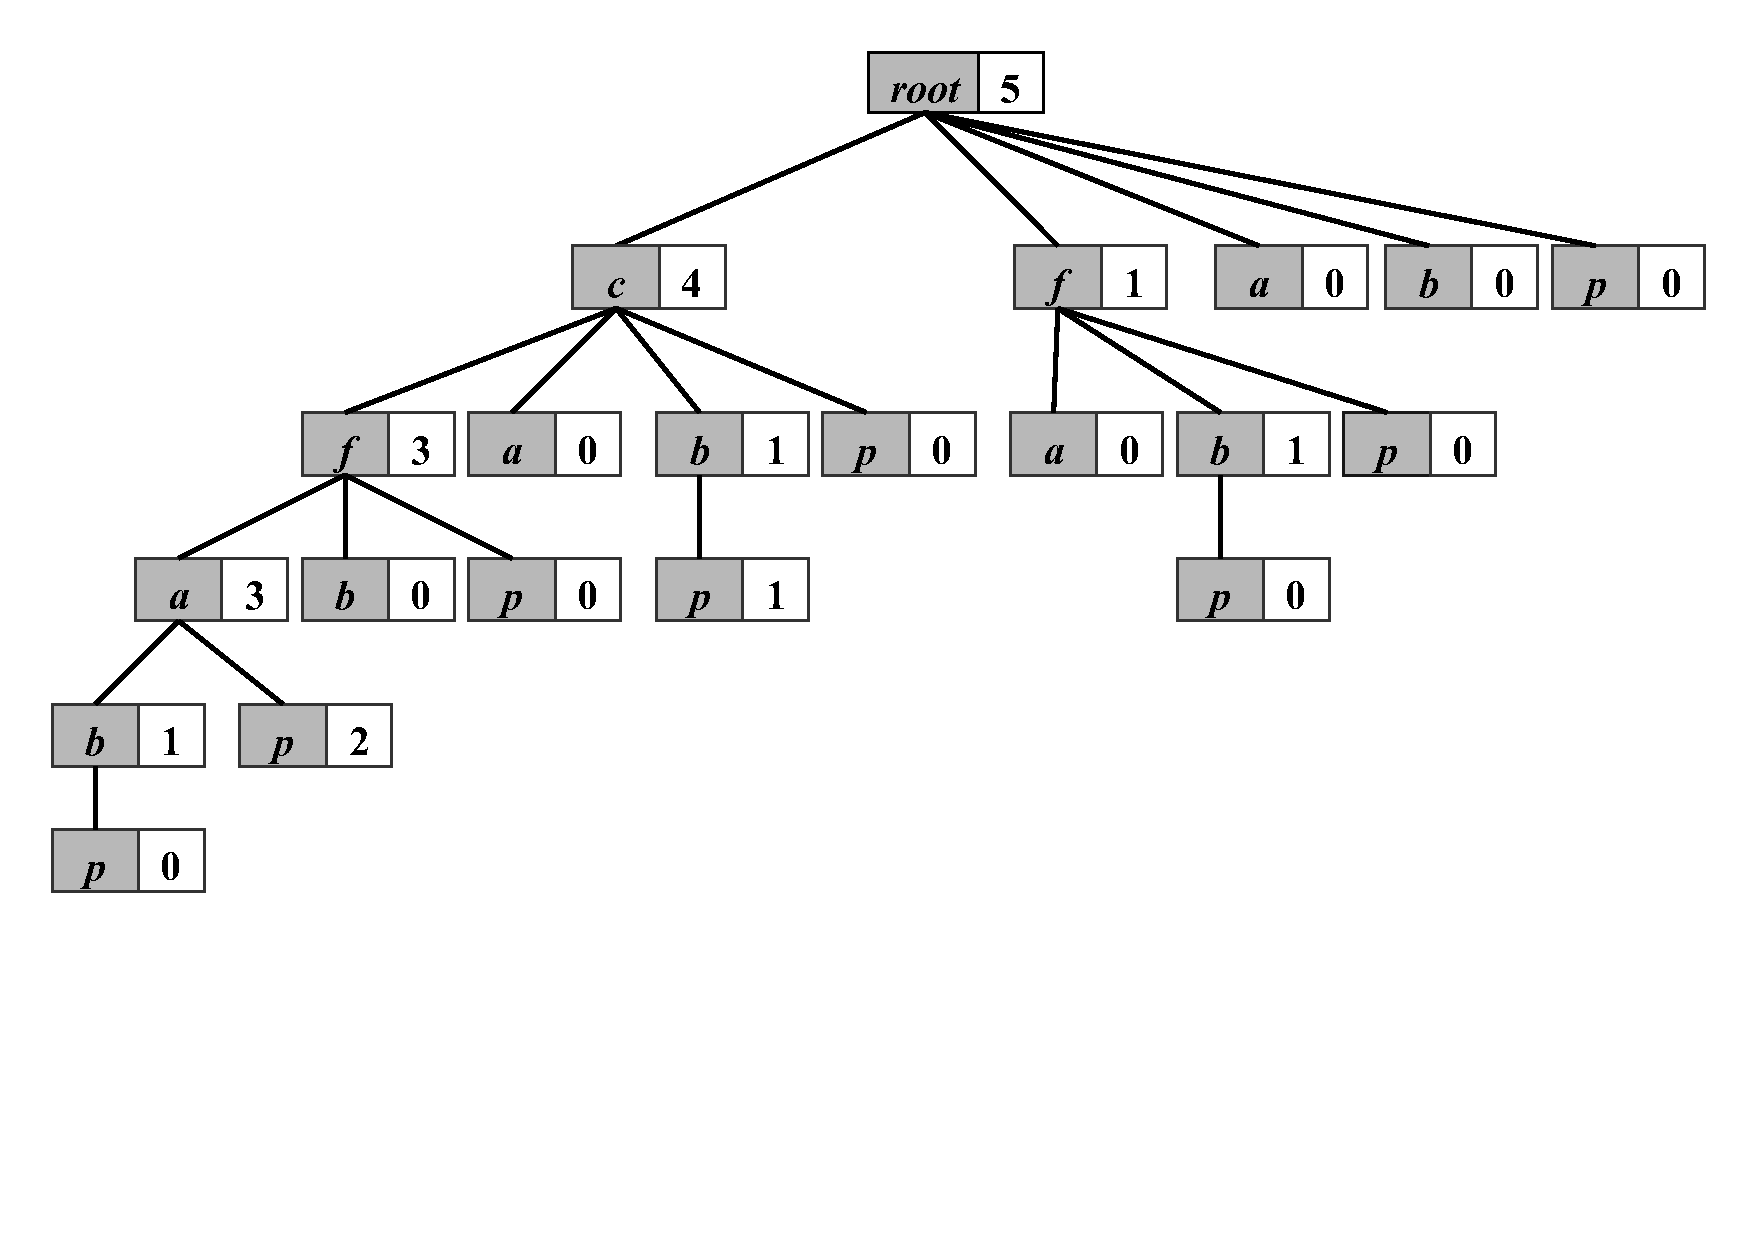
\includegraphics[width=0.8\textwidth]{fptree.pdf}
    \caption{模式树}
    \label{fig:fptree}
  \end{figure}

\subsection{本地化差分隐私(LDP)}
  FO协议

  PSFO协议


\section{本文工作}
\label{section:fullstep}
传统的FIM任务是不考虑用户隐私的,Apriori\cite{agrawal1994fast}和FP-growth\cite{han2000mining}等方法对用户原始数据挖掘且不加任何限制,极大的损害了用户利益。

为了充分考虑用户的个人隐私,本文使用本地化差分隐私机制聚合用户信息,并结合FP-growth方法\cite{han2000mining}的快速与高效性,提出并实现了一种基于本地化差分隐私的快速$top-k$频繁项集挖掘方法。总体框架见算法\ref{alg:fullstep}

\begin{algorithm}[htbp]
    \caption{总体框架}
    \label{alg:fullstep}
        \begin{algorithmic}[1]
        \REQUIRE ~~\\
        $n$位用户的交易数据集 $\mathrm{DB}=\left\{t_{1}, t_{2}, \ldots, t_{n}\right\}$;\\
        正整数$k$;隐私预算$\epsilon$;
        \ENSURE $top-k$的频繁项集
        \STATE 将数据集$DB$均分为两个组$D B_{1}$和$D B_{2}$;
        \label{fullstep:group}
			 \STATE $\tilde{S_k} = SVIM(DB_1,\epsilon,k)$; \ \  //SVIM\cite{wang2018locally}方法收集$top-k$的频繁$1-itemset$集合$\tilde{S_k}$
        \label{fullstep:SVIM}
			 \STATE $\tilde{IS_k} = minefp(DB_2,\epsilon,k,\tilde{S_k})$; \ \  //本文方案minefp,详见\ref{section:minefp}节
			 %\STATE 使用本文所提ldp-fp方案收集$DB_2$的信息,得到$top-k$的$\alpha -itemset$集合$\tilde{IS_k}$
			 \label{fullstep:minefp}
        \RETURN $\tilde{S_k} \cup \tilde{IS_k}$
        \end{algorithmic}
\end{algorithm}

本文在将FP-growth模式挖掘方法用于LDP场景时,所需要解决的问题主要有:

1、如何获得频繁$1-itemset$;

2、如何构建频繁模式树。

对于问题1,其等同于LDP的PSFO任务,本文使用文献\cite{wang2018locally}所提的SVIM方法,收集$top-k$的频繁$1-itemset$集合$\tilde{S_k}=\left\{x^{1}: \tilde{\theta}(x^1), x^{2}: \tilde{\theta}(x^2), \ldots, x^{k}: \tilde{\theta}(x^k)\right\}$,其中$\tilde{\theta}(x^i)$是项$x^i$的估计频数,$1\leq i \leq k$,更多算法细节参见文献;

对于问题2,通过分析,我们发现模式树的层次建立能够更好的契合LDP场景,提出minefp方案收集$top-k$的$\alpha -itemset(\alpha>1)$集合$\tilde{IS_k}$,详见\ref{section:minefp}节。

根据分析,整个机制是满足$\epsilon-LDP$的,不会泄露用户隐私。

\subsection{minefp方案介绍}
\label{section:minefp}
根据上述对总体框架的介绍可知,本文主要工作是提出了minefp方案用以收集$top-k$的$\alpha -itemset(\alpha>1)$集合$\tilde{IS_k}$。

\begin{algorithm}[ht]
    \caption{minefp}
    \label{alg:minefp}
        \begin{algorithmic}[1]
			 \REQUIRE ~~\\
			 数据集$DB_2$;\\
			 隐私预算$\epsilon$;\\
			 正整数$k$;\\
			 频繁$1-itemset$集合$\tilde{S_k}$;
			 \ENSURE $top-k$的挖掘结果$\tilde{IS_k}$
                 \STATE 预处理数据集$DB_2$,删除用户记录中的非频繁项目并重新排序;\\//预处理步骤
                 \label{minefp:preprocessing} 
                 \STATE 分配隐私预算$\epsilon_1 + \epsilon_2 = \epsilon$;
                 \label{minefp:epsilon}            
                 %\STATE 将$DB_2$按比例分为互斥的两组$transaction_1$和$transaction_2$;
                 %\label{minefp:group}
			 \STATE $iterNum = FO\_MaxIter(transaction_1,\epsilon_1)$; \\ //FO协议聚合transaction\_1中用户记录长度的信息,%详见算法\ref{alg:FO_MaxIter}
			 \label{minefp:iterNum}
			 \STATE $tree = build\_fpTree(transaction_2,\tilde{S_k},\epsilon_2,iterNum)$; \\ //层次构建频繁模式树,%详见算法\ref{alg:build_fpTree}
			 \label{minefp:tree}
			 \STATE $\tilde{IS} = FP\-growth(tree)$; \\ //FP-growth方法挖掘模式树tree
                 \label{minefp:fpgrowth}
			 \STATE 优化$\tilde{IS}$并选择$top-k$记为$\tilde{IS_k}$ \\ //后处理步骤,不消耗隐私预算
                 \label{minefp:optimize}
                 \RETURN $\tilde{IS_k}$
        \end{algorithmic}
\end{algorithm}
%算法中是分组  还是  分预算 最后要明确
%对上述算法简单介绍,引出下文

算法\ref{alg:minefp}描述了minefp方案的总体框架,首先对整个用户数据进行预处理并分配隐私预算(步骤\ref{minefp:preprocessing}、\ref{minefp:epsilon});然后为了建立频繁模式树,先聚合用户记录长度估计出树的最大层次(步骤\ref{minefp:iterNum}),最后以最大层次进行频繁模式树的层次建立(步骤\ref{minefp:tree});在建立模式树之后,挖掘出有效的频繁项集并且对结果进行一定的优化处理后发布(步骤\ref{minefp:fpgrowth}、\ref{minefp:optimize})。


\subsection{最大树层次}
\label{section:MaxIter}
本文是在LDP场景下层次建立频繁模式树,树的最大层次与隐私预算的分配直接相关。如图\ref{fig:fptree}所示模式树,最大层次为5。用户的记录长度是敏感信息,其长度不固定且具有随机性。

为了估计出有效的最大用户记录长度,本文使用FO协议对用户的长度进行一次聚合,并找到第80百分位长度值为$iterNum$,然后使用该值建立频繁模式树(\ref{section:buildTree})。

\begin{algorithm}[ht]
\caption{FO\_MaxIter}
\label{alg:MaxIter}
\begin{algorithmic}[1]
\REQUIRE 数据集$transaction_1$;\\
隐私预算$\epsilon_1$;
\ENSURE 最大迭代次数MaxIter

\STATE 初始化误差临界值$error = 3.0 \cdot \frac{\sqrt{n_1}}{\epsilon_1}$; //$n_1$为$transaction_1$的用户总数
\label{T threshold}
\STATE 对所有长度$l \in [1,2,\ldots,k]$以预算$\epsilon_1$使用FO协议聚合用户数$\Phi(l)$,并且剔除估计结果不大于$error$的项
\STATE 计算出$iterNum$使得$\frac{ \sum_{l=1}^{iterNum} \Phi(l)}{\sum_{l=1}^k \Phi(l)} > 0.8$成立;
\label{gamma=0.8}
\RETURN 最大迭代次数$iterNum$
\end{algorithmic}
\end{algorithm}

其过程与文献\cite{wang2018locally}中对$L$值的确定相似,本文对其中一些参数值做了修改,具体见算法\ref{alg:MaxIter}。

\subsection{层次建树}
\label{section:buildTree}
  本节详细介绍了minefp方案的具体建树过程,与FP-growth方法不同的是,本文在LDP场景下采用层次建树方式,构建模式树,如图\ref{fig:fptree}。具体步骤如下(详见算法\ref{alg:bulid tree}):(记树中根节点为第$level = 0$层,向下依次递增)

1、初始化树的根节点$root$,为树的$level=0$层;

2、第$level=1$层树节点聚合;对预处理后的交易记录进行一次LDP频率估计,如下

如用户$u_{1}$预处理后的交易为{\color{red}$c,f,a,p$},则其当前阶段的隐私信息为其前$level=1$个项,即为$c$;

用户$u_{2}$预处理后的交易为{\color{red}$c,f,a,b$},则其隐私信息为$c$;

用户$u_{3}$预处理后的交易为{\color{red}$f,b$},则其隐私信息为$f$;用户$u_{4}$的隐私信息为$c$;用户$u_{5}$的隐私信息为$c$。

则经过第三方聚合后,得到结果为$\{(c,4),(f,1)\}$,然后建第$level=1$层树节点,如图\ref{figure:levelone}所示,其中由于FO协议的特性,需要已知聚合的值域,也就是当前层的所有可能节点(见\ref{section:Q1}),图中计数为0的节点为无效节点。

  \begin{figure}[h]
    \centering
    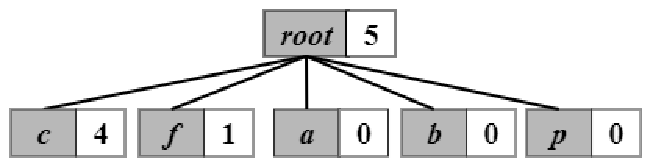
\includegraphics[width=0.6\textwidth]{level_1.pdf}
    \caption{第$level=1$层树节点}
    \label{figure:levelone}
  \end{figure}

3、第$level=2$层树节点聚合;

用户$u_{1}$预处理后的交易为{\color{red}$c,f,a,p$},则其当前阶段的隐私信息为其前$level=2$个项,即为$(c,f)$;

用户$u_{2}$的隐私信息为$(c,f)$,用户$u_{3}$的隐私信息为$(f,b)$,用户$u_{4}$的隐私信息为$(c,b)$,用户$u_{5}$的隐私信息为$(c,f)$

第三方聚合结果为$\left \{ (c,f,3) , (c,b,1) , (f,b,1) \right \}$,根据路径建立第$level=2$层树节点,如图\ref{figure:leveltwo}所示:

  \begin{figure}[h]
    \centering
    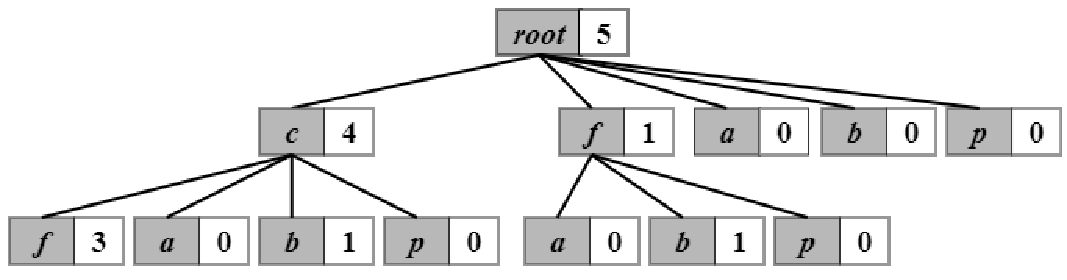
\includegraphics[width=0.8\textwidth]{level_2.pdf}
    \caption{第$level=2$层树节点}
    \label{figure:leveltwo}
  \end{figure}

4、依层次$level$递增顺序,直到达到树的最大层数,建立模式树如图\ref{fig:fptree}所示。

%建树算法修改
\begin{algorithm}[ht]
\caption{build\_tree}
\label{alg:bulid tree}
\begin{algorithmic}[1]
\REQUIRE ~~\\
数据集$transaction_2$;\\
$top-k$频繁$1-itemset$集合$\tilde{S_k}$;\\
隐私预算$\epsilon_2$;\\
最大层数$iterNum$;
\ENSURE 模式挖掘结果$\tilde{IS_k}$
\STATE 初始化树根结点$root$为空;
%\STATE 分配隐私预算$\epsilon^{\prime} = \epsilon_2 / iterNum$;
\FOR{层次$j=1$ to $iterNum$}
    \STATE 均匀分配隐私预算为$\epsilon^{\prime}$;
    \label{tree:epsilon}
    \STATE 根据第$j-1$层保留的树节点生成孩子为第$j$层树节点,并初始化节点计数为0;
    \label{tree:child node}
    \STATE 以预算$\epsilon^{\prime}$使用FO协议聚合得到第$j$层节点信息信息;
    \label{tree:FO}
    \STATE 初始化误差临界值为协议标准差$standard\_error$;
    \label{tree:error bound}
    \STATE 删除估计的计数值不大于$standard\_error$的节点;
    \label{tree:filter}
    \STATE 一致性约束并更新节点信息;
    \label{tree:consistency and update}
\ENDFOR
\RETURN $root$
\end{algorithmic}
\end{algorithm}

% 对算法中的具体过程详细介绍!!!!!因子这是本文的主要贡献——将Q1至Q4具体介绍

算法\ref{alg:bulid tree}介绍了层次建树的基本流程,其中步骤\ref{tree:epsilon}至步骤\ref{tree:update}介绍了树层次节点的建立与信息更新。为了保证模式树的有效性与完整性,在使用LDP协议聚合用户信息以及更新树中节点时,需要对具体步骤进行细节优化。以下详细介绍了算法中的各步骤及其优化过程。

\section{建树优化}

\subsection{隐私预算分配}\label{section:Allocate privacy budget}
层次建树过程中,本文均分隐私预算对树的层次节点LDP聚合。若给定最大层次$iterNum$(见\ref{section:MaxIter}节),共计有两种预算分配方式:

a、将$\epsilon$均分为$\epsilon^{\prime} = \epsilon / iterNum$,所有用户共计参与LDP聚合$iterNum$次;

b、将数据集均分为$iterNum$组,每组使用全部隐私预算$\epsilon^{\prime} = \epsilon$参与其中一次LDP聚合,且不重复参与。

文献\cite{wang2018privtrie,wang2018locally}表明,分配方式b优于方式a,且能有效降低$O(\sqrt{iterNum})$倍误差。

本文在实验中,均使用方式b分配隐私预算。

\subsection{层次节点初始化}
  在使用FO协议聚合第$j$层节点信息时,根据FO协议特性,其输入输出值域$I$和隐私预算$\epsilon$需要是已知的。对于隐私预算的分配,见\ref{section:Allocate privacy budget}节,故而本节主要介绍协议在第$j$层聚合时,输入输出值域$I_j$的确定以及优化。

  \textbf{基本方法}
  根据模式树层次建立的特性,第$j$层的节点信息,不仅与FO协议的聚合结果相关,而且与第$j-1$层保留的节点有关(因为无效节点——节点计数为0——不会生成孩子节点)。所以,一种生成$I_j$的直接方法是根据上一层(第$j-1$层)保留的节点,生成其所有可能的孩子节点作为初始值域$I_j$,用以FO协议聚合。

  以图\ref{fig:fptree}模式树为例,根节点$root$为第$j=0$层;

  当$j = 1$时,其上一层为根节点,则$I_1$初始为$\tilde{S_k}$中所有的频繁项目,即$I_1 = \left\{ (c), (f), (a), (b) , (p)\right\}$;设此时FO协议聚合结果为$\{(c,4),(f,1)\}$,则保留节点$\left\{ (c), (f)\right\}$为有效节点。

  当$j = 2$时,第$j = 1$层保留的有效节点为$\left\{(c),(f) \right\}$,则所有可能的孩子节点路径为$\left\{(c,f),(c,a),(c,b),(c,p),(f,a),(f,b),(f,p)\right\}$即为$I_2$;(孩子节点生成规则:根据$\tilde{S_k}$的项目顺序$c,f,a,b,p$,保证模式树中的节点的孩子所对应项目,其次序要小于其父节点对应项目的次序)。

  同理可得,$I_3 =\left\{(c,f,a),(c,f,b),(c,f,p),(c,b,p) \right\}$;\\$I_4 = \left\{ (c,f,a,b),(c,f,a,p)\right\}$ ;$I_5 = \left\{ (c,f,a,b,p)\right\}$ 。

  \textbf{优化方法}
  上述基本方法的缺点在于,当$\tilde{S_k}$中确定的频繁项目较多或者上一层有效节点个数较多时,所生成的孩子节点会明显增多,从而使得值域$I_j$较大(即$|I_j|$较大)。而根据FO协议的特性,其估计误差与$| I_j |$直接相关,如GRR方法的估计方差与$d_j$呈线性关系,尽管OLH方法的方差与$|I_j|$无直接关系,但是其使用了$hash$函数将$|I_j|$映射至$g = \left \lceil e^{\epsilon}+1 \right \rceil$,随着$|I_j|$的增大,在统计聚合时,会导致$hash$碰撞明显增多,从而准确度降低。
 
  为了有效缩小$|I_j|$,从而提高估计准确度,本文提出值域筛选方法,能够在不影响结果准确性的同时将$I_j$限制在大小为$3k \ll |I_j|$范围,且整个过程不消耗隐私预算。

\begin{algorithm}[h]
\caption{prune candidate}
\label{alg:prune candidate}
\begin{algorithmic}[1]
\REQUIRE ~~\\
候选值域$I_{j}$;\\
$top-k$的$\tilde{S_k}$;\\
正整数$k$;\\
参数$\xi$;
\ENSURE 筛选后值域$I^{\prime}_{j}$

\IF{$ | I_{j} |$不大于$\xi \cdot k$}
    \STATE $I^{\prime}_{j} = I_{j}$;
\ELSE
    \STATE 初始化$I^{\prime}_{j} = \emptyset$;
    \FOR{each 候选值$X \in I_{j}$}
        \STATE $\varphi(X)=\prod_{x \in X} \tilde{\theta}(x)$;    //$\tilde{\theta}(x)$表示$\tilde{S_k}$中项目$x$的估计频数。\label{prune:speculate the frequency}
        \STATE $I^{\prime}_{j} = I^{\prime}_{j} \cup X$,并且记录$\varphi(X)$
    \ENDFOR
    \STATE 以$\varphi(X)$为标准,将$I^{\prime}_{j}$排序,最后选择前$\xi \cdot k$个赋值给$I^{\prime}_{j}$
\ENDIF

\RETURN $I^{\prime}_{j}$
\end{algorithmic}
\end{algorithm}

  算法\ref{alg:prune candidate}给出了值域筛选的具体过程,其中步骤\ref{prune:speculate the frequency}类似于文献\cite{wang2018locally}所提SVSM的推测频率方法,而在本算法中,候选值$X$中项目个数是相同的,故而本算法对项目频数直接相乘即可得到相对排序。

  参数$\xi$用以调节值域大小,呈线性正相关。本文在实验中选用$\xi = 3$,能够有效权衡误差与准确度($\xi$越小,则值域越小,有可能会使得舍弃大量的有效信息,降低准确度)

\subsection{筛选有效聚合结果}
  通过算法\ref{alg:prune candidate}得到$I_j$之后,根据路径生成相应的树节点即为第$j$层初始节点,使用FO协议进行信息聚合。当某用户在当前阶段的记录项目个数小于层次$j$或所得值域$I_j$中不包含用户的记录对应的路径,那么,则该用户以无效值$\perp$为原始数据参与聚合。此时的值域应为$I_j \cup \perp$,其大小为$\xi \cdot k + 1$

  然而,由于LDP协议的存在估计误差,聚合结果中存在无效的估计值(如估计值不大于0等),应当在保留有效估计的同时,尽可能多的舍去无效估计。

  \textbf{(类似误差值的设置有三种方法:)}

1)、$standard\_error = \sqrt{Var}$,即标准差;

2)、文献\cite{wang2017locally,wang2018locally},$standard\_error = \mathrm{T}=F^{-1}\left(1-\frac{0.05}{2 k}\right) \sqrt{Var}$,$F^{-1}$为标准正态分布的CDF的倒数;

3)、文献\cite{wang2018privtrie}根据伯恩斯坦不等式求得最大误差边界,从而设置误差值。

  为了简化操作,本文在建树过程中,设置误差值为协议的估计标准差,将所得估计值不大于标准差的项视为无效估计,舍弃。

\subsection{一致性约束}
\label{section:consistency}
  设$v$表示树中某节点,其相应的计数值为$v.count$,$\tilde{C}(\cdot),C(\cdot)$分别表示估计值与真实值,则对于节点$v$应有以下约束规则:

  1)、无偏估计:$\mathbb{E} \left [ \tilde{C}(v.count) \right ] = \mathbb{E} \left [ C(v.count) \right ]$;即对节点的计数值的估计保证无偏(FO协议)。

  2)、父节点计数值不小于孩子节点计数之和:记$v.children$表示$v$的所有孩子节点集合,假设共有$r$个孩子:\\
  $$\mathbb{E} \left [ \tilde{C}(v.count) \right ] \ge \sum_{y \in v.children} \mathbb{E} \left [ \tilde{C}(y.count) \right ] \eqno{(11)}$$

  约束推理规则是后处理步骤,能够有效提高结果的准确性, 文献\cite{hay2010boosting,wang2018privtrie,lee2014top}等均研究了不同场景下的约束推理方式,其中文献\cite{wang2018privtrie}对两次的聚合结果进行矫正,不适用于本文场景;而文献\cite{hay2010boosting,lee2014top}均是DP机制下的约束推理。

  在本文中,利用文献\cite{hay2010boosting}思想,采用以下方式对结果进行约束

  \textbf{具体矫正步骤——{\color{red}unsure}}:

  设$Y = (y_{1},y_{2},\ldots ,y_{r})$表示节点$v$的所有孩子节点(共$r$个)相应计数值,矫正的目的在于计算新的向量$Y^{\prime}$使其与$Y$的L2范式最小(文献\cite{hay2010boosting,lee2014top}),形式化表示为:
  
  $$\underset{Y^{\prime}}{\text{minimize}}  \left \| Y^{\prime} - Y \right \|^{2}_{2} \  ,\  subject to \left \| Y^{\prime} \right \| = v.count\eqno{(12)}$$

  上式可根据拉格朗日求解法得到$Y^{\prime} = Y - \frac{1}{2}A \ , \ A = \frac{2(\sum{i=1}^{k}y_{i} - A)}{r}$,其中$r$表示$v$的孩子节点总个数,而$A = v.count$。

  即,在更新当前第$j$层树节点的之后,若对于$j-1$层存在违背约束的节点,则根据上述结果进行一致性矫正。

\section{结果优化}
\label{section:optimize}

\section{实验}


%设置文献的样式
\bibliographystyle{plainnat}      %unsrt表示PDF文末的参考文献列表是按照文中的引用顺序排序
%添加自己的bib文件
\bibliography{reference} 
\end{document}